\newcommand{\plugtext}[1]{\texttt{\normalsize{#1}}}

\begin{tikzpicture}
    \begin{scope}[x={(0mm,135mm)},y={(0mm,79mm)},line width=1pt,cap=round]
        %\node[anchor=south west,inner sep=0mm] at (0mm,0mm) {\includegraphics[width=135mm]{images/pcb/pcbOverviewBWHL.jpeg}};
        \node[anchor=south west,inner sep=0mm] at (0mm,0mm) {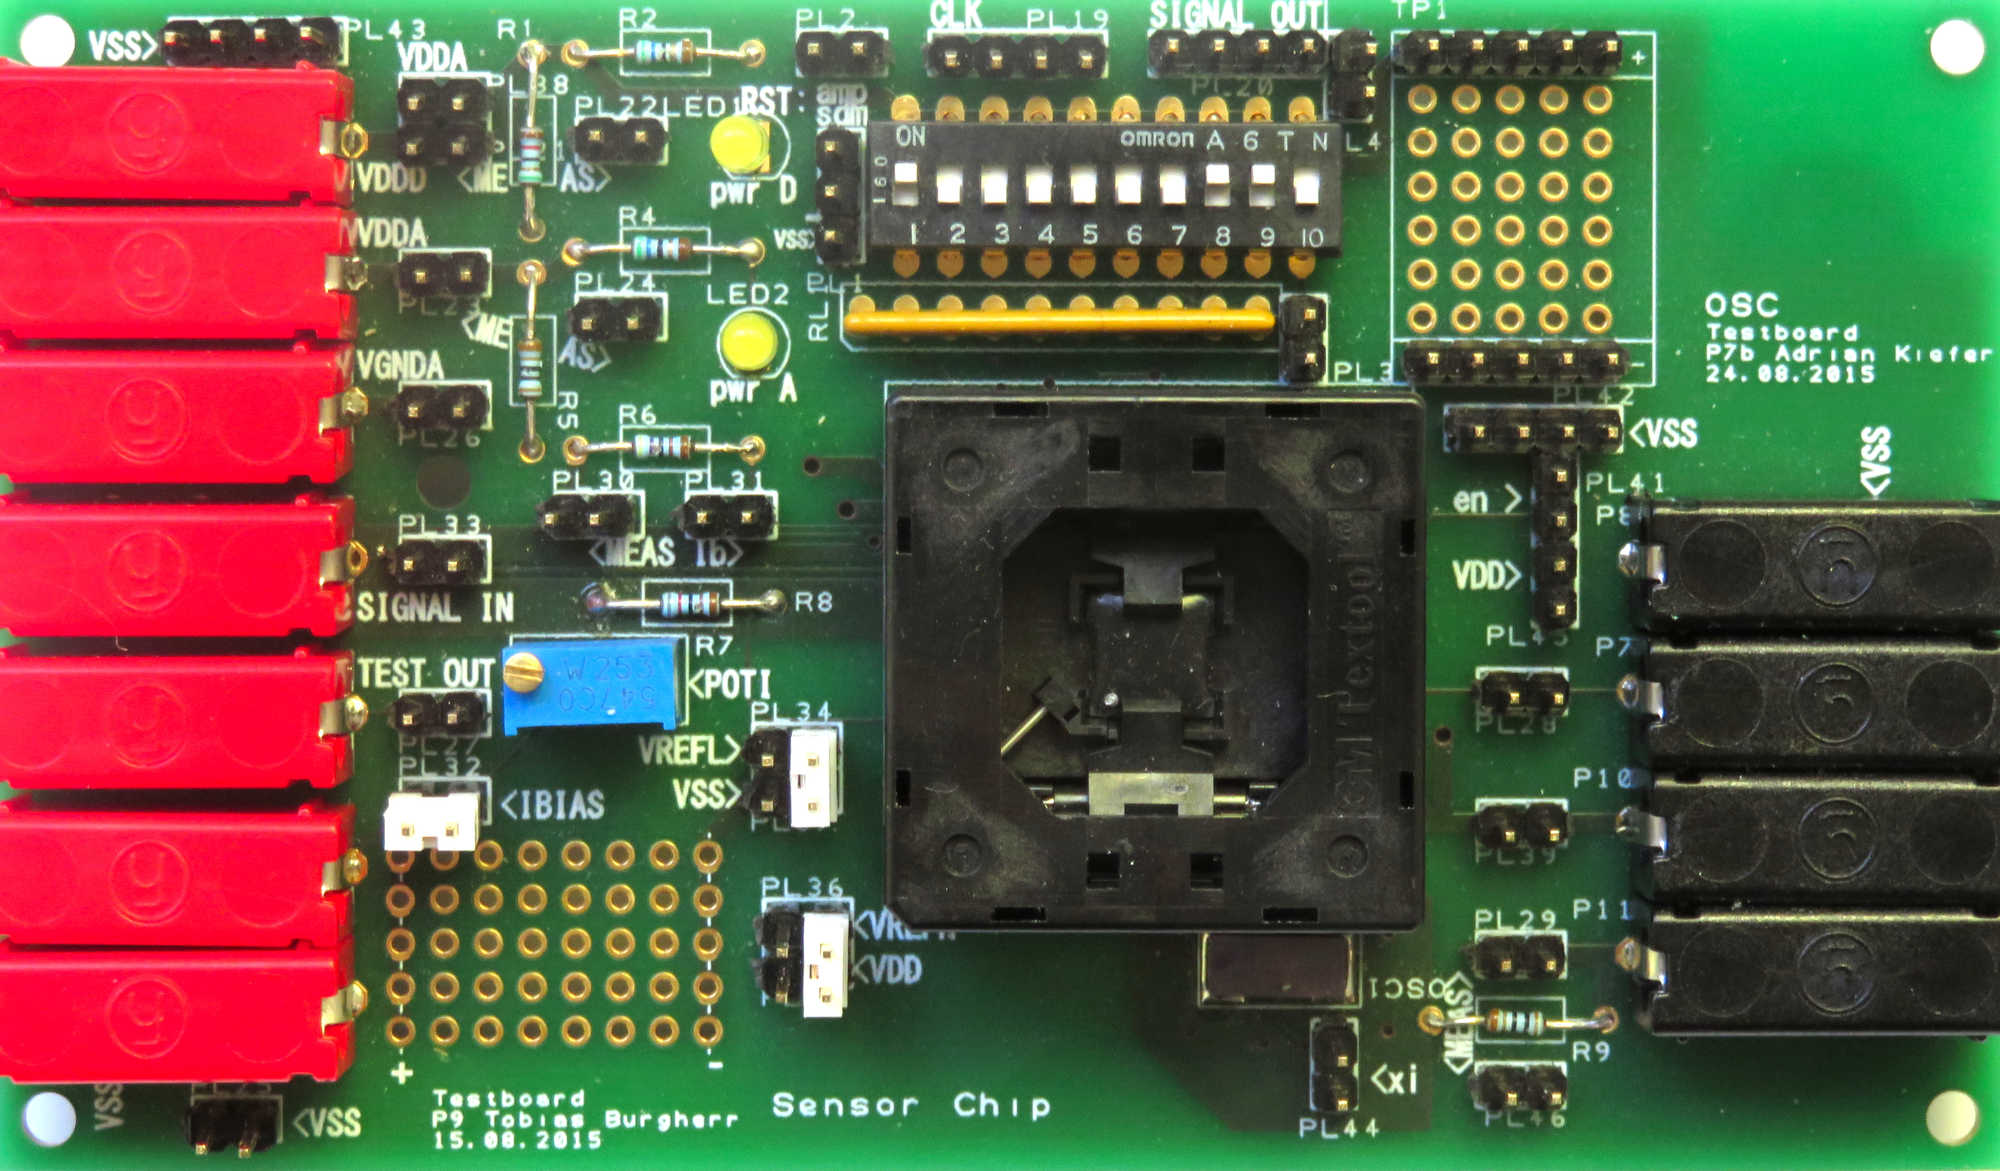
\includegraphics[width=0.75\textwidth]{images/pcb/pcbOverview.jpeg}};
    \end{scope}
    %\node[fill=black,text=black,anchor=south west] at (0mm,0mm) {\textsf{\Large{VDDD}}};

    \node[%
        text=black,
        anchor=south east] at (-1mm,52mm) {\plugtext{VDDD}};

    \node[%
        text=black,
        anchor=south east] at (-1mm,44mm) {\plugtext{VDDA}};

    \node[%
        text=black,
        anchor=south east] at (-1mm,37mm) {\plugtext{VGNDA}};

    \node[%
        text=black,
        anchor=south east] at (-1mm,29mm) {\texttt{SIGNAL IN}};

    \node[%
        text=black,
        anchor=south east] at (-1mm,21mm) {\texttt{TEST OUT}};

    \node[%
        text=black,
        anchor=south east] at (-1mm,13mm) {\plugtext{IBIAS}};

    \node[%
        text=black,
        anchor=south east] at (-1mm,5mm) {\plugtext{VSS}};

    \node[%
        text=black,
        anchor=south east] at (55mm,62mm) {\rotatebox{90}{\plugtext{CLK}}};

    \node[%
        text=black,
        anchor=south east] at (67mm,62mm) {\rotatebox{90}{\plugtext{SIGNAL OUT}}};
\end{tikzpicture}
